\documentclass[class=book, crop=false]{standalone}

%% Image paths
\usepackage{graphicx}
\graphicspath{{images/}}

%% Language and font encodings
\usepackage[english]{babel}
\usepackage[utf8x]{inputenc}
\usepackage[T1]{fontenc}
\usepackage{csquotes}

%% Sets page size and margins
\usepackage[a4paper,top=3cm,bottom=2cm,left=3cm,right=3cm,marginparwidth=1.75cm]{geometry}

%% Sets epigraph style
\usepackage{epigraph}
\setlength\epigraphwidth{.8\textwidth}
\setlength\epigraphrule{0pt}

%% Sets line style
\linespread{1.3}

%% Key term command
\usepackage{marginnote}
\providecommand{\keyterm}[1]{\textbf{#1}\marginnote{\scriptsize \textbf{#1}}}

\begin{document}

\epigraph{\itshape “Rules broken today become norms tomorrow.”}{---Bill Gates}

In June of 2009, former Facebook CTO Adam D'Angelo and former Facebook manager Charlie Cheever co-founded a simple question-answering site called Quora\index{Quora}. Quora didn't look very different from its competitors such as Yahoo Answers\index{Yahoo Answers}, Reddit and Google's Aardvark. From a technical point of view, there was nothing special about Quora.

However, Quora exploded onto the market. So many users joined that Quora had trouble keeping the site up at times. And even before it was released to the general public, Quora was valued at 86 million dollars. Today, Quora is valued at 2 billion dollars.

So why was Quora so popular? Unlike its competitors, Quora gained a reputation for high-quality answers, many of them from experts in their fields. For example, Facebook co-founder Dustin Moskovitz answered a question about the Facebook film \textit{The Social Network}. The product manager of Google Images answered a question about how color image searches work. Former AOL CEO Stephen Case answered a question about the cost of mailing CDs to potential customers in the nineties. [Arthur and Kiss 2011]

\begin{figure}[!tbp]
  \centering
  \begin{minipage}[b]{0.4\textwidth}
    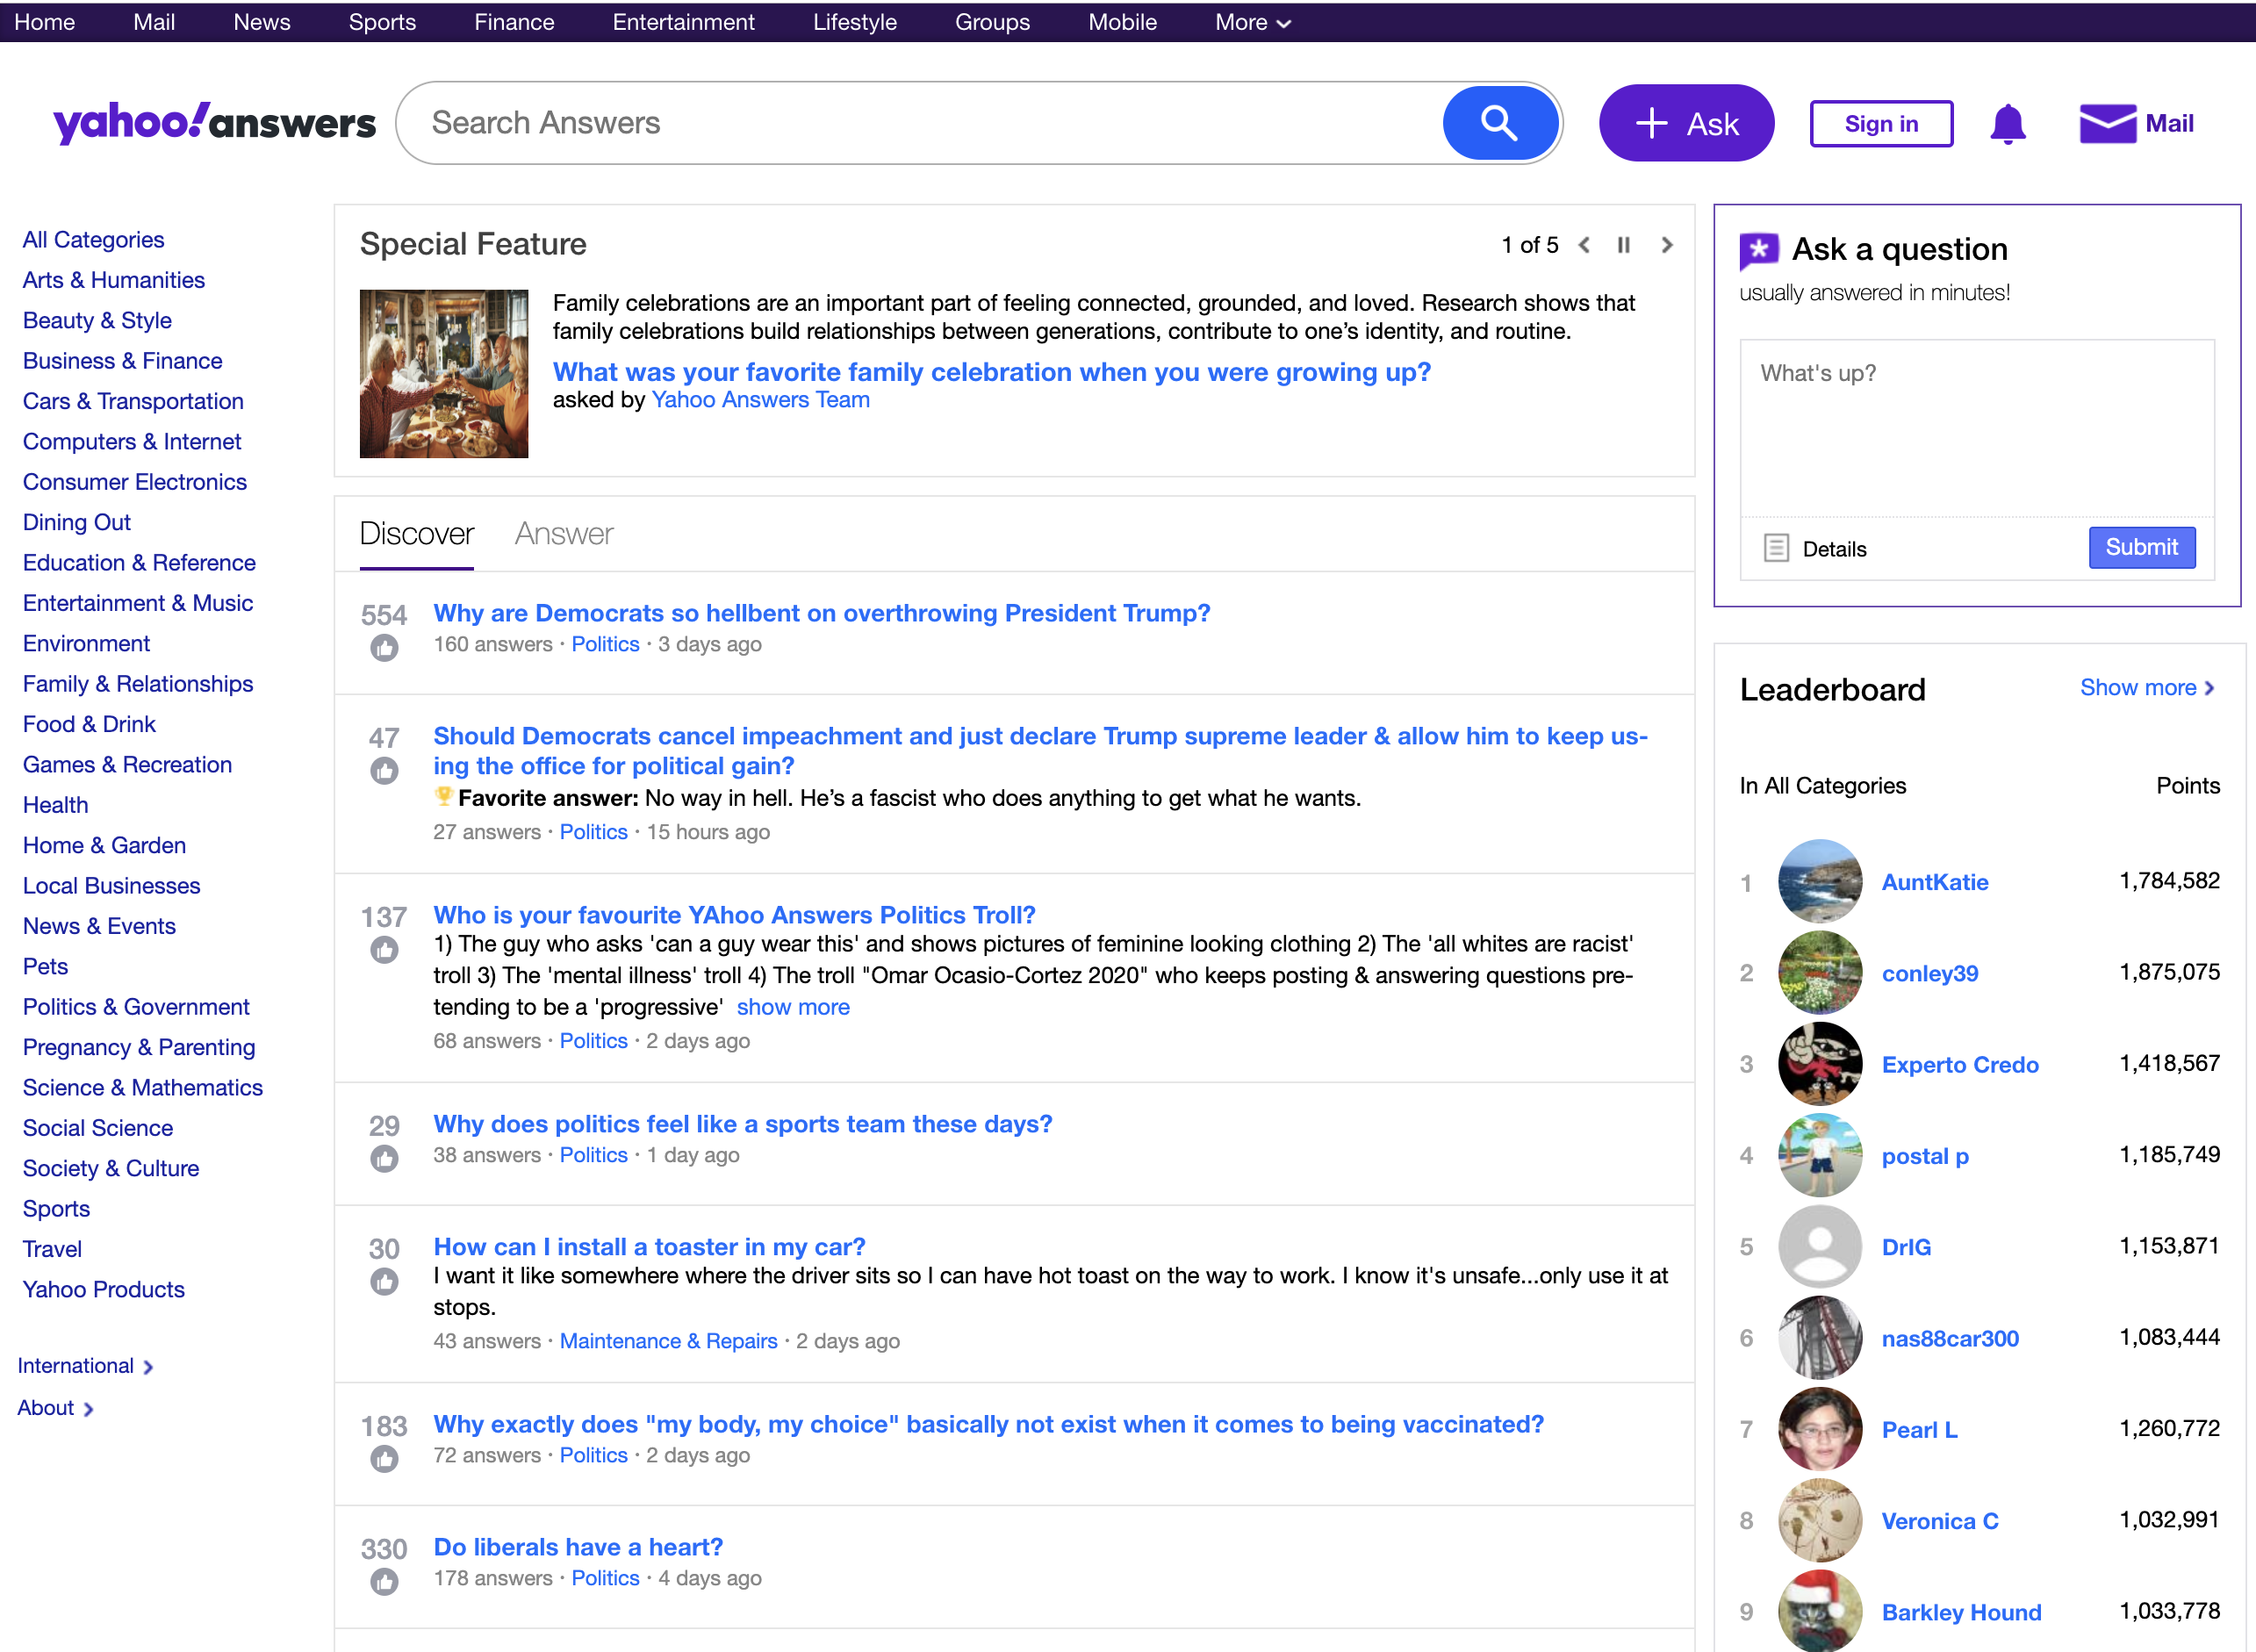
\includegraphics[width=\textwidth]{yahooanswers}
    \caption{Yahoo Answers}
  \end{minipage}
  \begin{minipage}[b]{0.4\textwidth}
    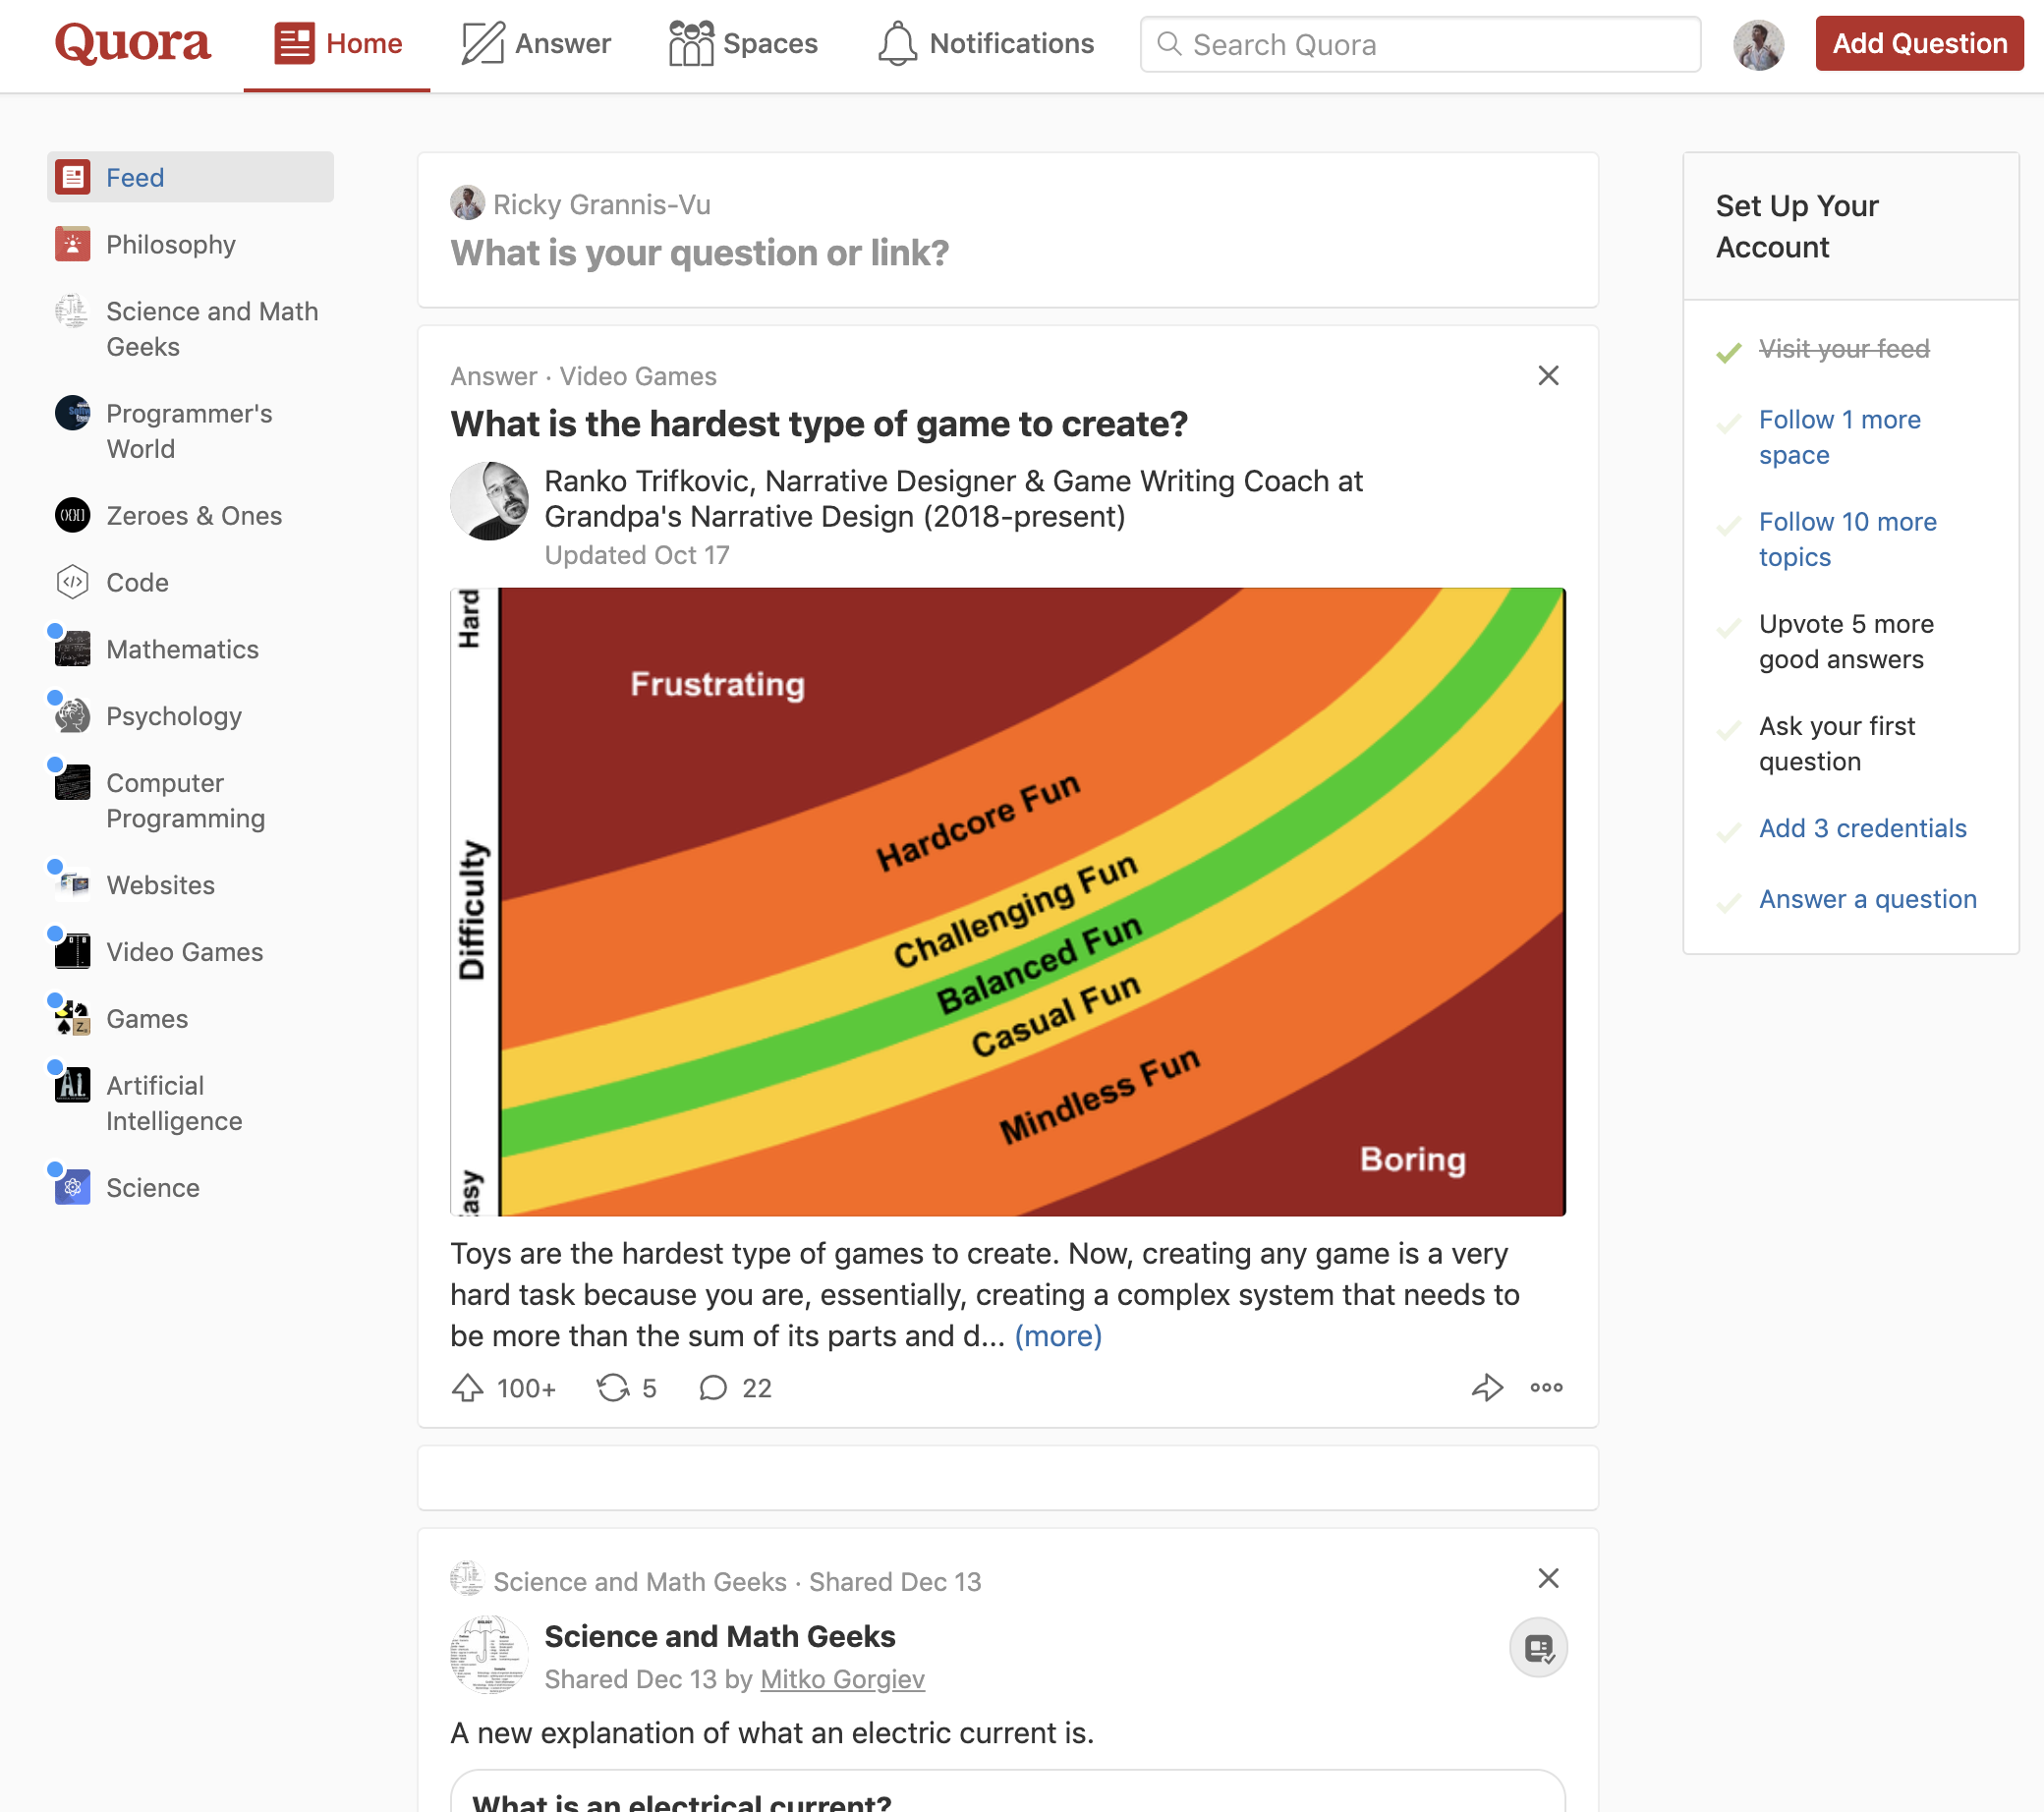
\includegraphics[width=\textwidth]{quora}
    \caption{Quora}
  \end{minipage}
\end{figure}

Theodore Schleifer, writing for \textit{Vox}, described Quora\index{Quora} as "a more organized Yahoo Answers, a classier Reddit, an opinionated Wikipedia." Alyson Shontell, writing for \textit{Business Insider}, noted that "Quora stands out with its contributors -- the people answering questions on the site."

\section{Norms and culture}

Quora\index{Quora} was successful not because of its technical capabilities but because it established a positive \keyterm{culture}\index{culture}. A social system's culture is its collection of \keyterm{norms}\index{norm}, which are rules, often unwritten, which govern the behavior of the social system's participants. We can identify three different norms which led to Quora's success.

First, Quora has a norm of sourcing claims, often providing citations. This helped Quora avoid becoming overly opinionated, ensuring that all answers remained factual and, for the most part, objective.

Second, Quora has a norm of providing long and thought-out answers. This differs from answers on Yahoo Answers, which often take the form of brief sentences or paragraphs, and consequently often don't fully answer the questions.

Third, Quora\index{Quora} has a norm of well-written prose. Answers on Quora are easy to read because of their attention to English grammar and well-formed sentences. In addition, because contributors on Quora are paying closer attention to their grammar, they are more likely to spot potential errors in their reasoning, further boosting the quality of their answers.

The norms and culture of a social system have a huge effect on how the social system functions. For example, most adolescents use Instagram to publicly share selected aspects of their lives. Adolescents use Snapchat to share personal or humorous aspects of their lives. Adolescents use Facebook\index{Facebook} less than either Instagram or Snapchat, viewing it's design as too complicated and it's demographic as being too old for them. [Throuvala et al. 2019]

It's important to note that norms are \textit{not} universal. What is acceptable in one community might not be acceptable in another. Similarly, what is unacceptable in one community might even be expected in another. The way you choose your norms depends entirely on how you want your community to be used. Do you want your community to be known for objectivity and factual content? Then, you might institute a norm of peer review. Do you want your community to allow anybody to express their opinion freely? A norm of peer review would work against this goal.

Each norm can be thought of as bounding a subset of Internet users for your community. If you establish a norm of peer review, then users who want to freely express themselves might avoid your community. However, at the same time, establishing a norm of peer review will make users who want objective, factual content will be more inclined to use your site. This is the trade-off you must consider when choosing norms: you must find a balance between the number of targeted users and the relevance of the interactions between your users to your community's goal. If you establish too many norms, then you might reduce your targeted users to low levels and make the community unsustainable. If you establish too few norms, then your community might become derailed from its intended purpose.

We need norms. But we don't want superfluous norms -- every norm we create must have a purpose and it must actively further the community toward that purpose. Furthermore, we might want to establish a norm only if it \textit{significantly} furthers our community's purpose. Establishing a norm superfluously or which has low impact not only reduces the number of targeted users; it might also make the experience of engaging with the community less satisfying to those users still in it. We tend to chafe under norms which don't seem to be effective; users might feel that the community is too authoritarian or repressive and engage with the community less or be less helpful in the community.

So how do we test our norms? What most companies do when rolling out a new norm is that they test new norms \textit{one at a time} and they only test norms on a \textit{small subset of users}. For example, many tech companies roll out new norms to their employees first or to a limited beta group of users. In 2019, Instagram tested removing the like count from public posts. They didn't roll out the new norm to all their users at once. Instead, they tested on increasing sizes of users

Whichever norms we end up choosing, what is important is that we establish our norms early so that we don't have to try to change them later on, after they have been ingrained in the community.

\section{Injunctive and descriptive norms}

So how do we go about actually establishing a norm? Well, first, we need to be aware that there are two different types of norms that can be established.

The first type of norm is the \keyterm{injunctive norm}\index{norm!injunctive}. An injunctive norm describes what behavior is acceptable and what behavior is not acceptable. In an online community, this might take the form of a list of rules which members agree to abide by. Failure to abide by the rules might result in social isolation, loss of privileges or even account termination.

The second type of norm, a \keyterm{descriptive norm}\index{norm!descriptive}, on the other hand, describes what actually occurs in practice. For example, in an online community a new member might see that all members close their messages in a certain way. While the member might not be required by any rule to do the same, the member might still feel pressure to close their messages the same way in order to fit in.

Should we use descriptive or injunctive norms? The downside of making every norm descriptive is that it can lead to a long winding list of text (read the Facebook Code of Conduct sometime to get an idea of what this can look like). If the list of norms gets too long, then people simply won't read it. When was the last time you read the Terms of Service before downloading an update? Have you ever read it?

However, not making a norm descriptive can also have its drawbacks. For example, new members may not know the norms of a community or, at least, they may not appreciate the importance of the norms for the community [Kiesler et al. 2011]. And, furthermore, not all members may be able to derive norms from social cues online. For example, users with Asperger's Syndrome often struggle to infer social norms even after witnessing lots of others comply with thee norms. These users may fall afoul of a community's norms simply because they don't know what the norms are. [Burke et al. 2010]

Lampe, C et al. 2014. "Crowdsourcing Civility: A Natural Experiment Examining the Effects of Distributed Moderation in Online Forums." Government Information Quarterly 31 (2). Elsevier Inc.: 317-26.\\
 * Difficulty for newcomers learning norms can lead to high drop-out rates.

Matias, J.N. 2016b. "Posting Rules in Online Discussions Prevents Problems \& Increases Participation." CivilServant.\\
 * Making rules more visible may have a positive effect on newcomer participation.

\section{Defaulting}

Suppose you build a messaging app and provide a feature for users to receive new messages as an email digest in the morning. You set the feature to be off by default (you don't want your users complaining about spam!) but users can turn the feature on from your app's setting screen. That way, anybody who wants an email digest can get it.

Interestingly enough, many users might want an email digest but not turn the feature on. In 2011, Jared Spool designed an experiment to test whether users changed their defaults. He and his team found several hundred people who were willing to send them their settings for Microsoft Word (a file named config.ini). They analyzed all the files and found that less than 5\% of the users had changed any of their Microsoft Word settings. It is important to note, however, that almost all the users surveyed who were programmers and designers changed their settings. As a programmer or designer, remember that just because you change your settings doesn't mean everybody else does!

So why didn't most users change their settings? Many of the features turned off were really useful. For example, Microsoft Word by default made users manually save their documents; however, users could turn an autosave feature on in their settings file. But most users hadn't turned on the feature. As several participants said, "Microsoft must know what they are doing." (In fact, the feature was turned off because a programmer had decided to initialize all the options in the config.ini file with zeroes because it was easy to do so and no one ever told him otherwise. So much for Microsoft's knowing what they were doing!)

The default had become a sort of norm -- an understanding that the settings (thought to be) carefully curated and set to defaults by Microsoft were the normal ones and therefore the optimal choice. This plays out in a lot of online communities -- in the absence of clear direction on what a user should do, the user often regresses to relying on the defaults. Through this, \textit{defaults become norms}.

When users rely too heavily on default behaviors in an online community (a phenomenon called \textbf{defaulting}), things can get ugly. Default behaviors arise out of the \textit{absence} of clear community norms -- and many of them aren't healthy. For example, without community norms encouraging people to be respectful and civil towards each other, people might regress towards an undesirable default -- name-calling and insults (as often happens on certain message boards).

Take Microsoft Tay\index{Microsoft!Tay} for example, a Twitter chatbot which Microsoft released to the public in 2016. Tay promised “conversational understanding” -- it learned how to converse from the users it talked to. However, no norms were set about what users could do with Tay. In the absence of such norms, Tay soon became reflective of the worst parts of the Internet. Trolls fed Tay with misogynistic, racist and anti-Semitic remarks and within less than 24 hours, Tay was spouting sentences such as “Hitler was right I hate the jews” and “I f*cking hate feminists and they should all die and burn in hell.” Microsoft ultimately ended up having to shut down Tay. [Vincent 2016]

In summary, when designing an online community, make sure to set enough norms (but proper norms!) so that users don't rely on default behaviors. Default behaviors can often get pretty nasty -- and they have no place in your community!

\section{Changing norms}

Once a norm has become entrenched in your community, if you suddenly decide that your community won't abide by that norm anymore or that it will abide by a modified or opposing norm, your community will experience (potentially severe) fallout. This is commonly known as the \keyterm{ripple effect} -- decisions made early on, such as setting norms, can have huge consequences later on. This is why it's especially important to be aware of how your community's norms develop early on, so that you aren't forced to change any of the norms later.

For a good example of this, consider YouTube and its "Adpocalypse". When YouTube began, its goal was simple: to create a platform that anybody could use to upload videos about anything they wanted. In a world where you could only share videos through official outlets like Hollywood, YouTube was a way for everybody else to share. [Alexander 2019] As Alkhatib and Bernstein describe in their 2019 paper, YouTube had a norm of "free performance".

However, as the community became larger, YouTube was forced to address the dark side of its platform. Its original goal, letting \textit{anybody} share videos, became a problem. Terrorists posted recruitment videos on its site and YouTube ran ads on those videos, angering its advertising partners, who threatened to leave the platform. To try to prevent its partners from leaving, YouTube implemented a policy of demonetizing videos which advertising partners might view as problematic. [Alexander 2019]

\begin{figure}[!tbp]
  \centering
  \begin{minipage}[b]{0.4\textwidth}
    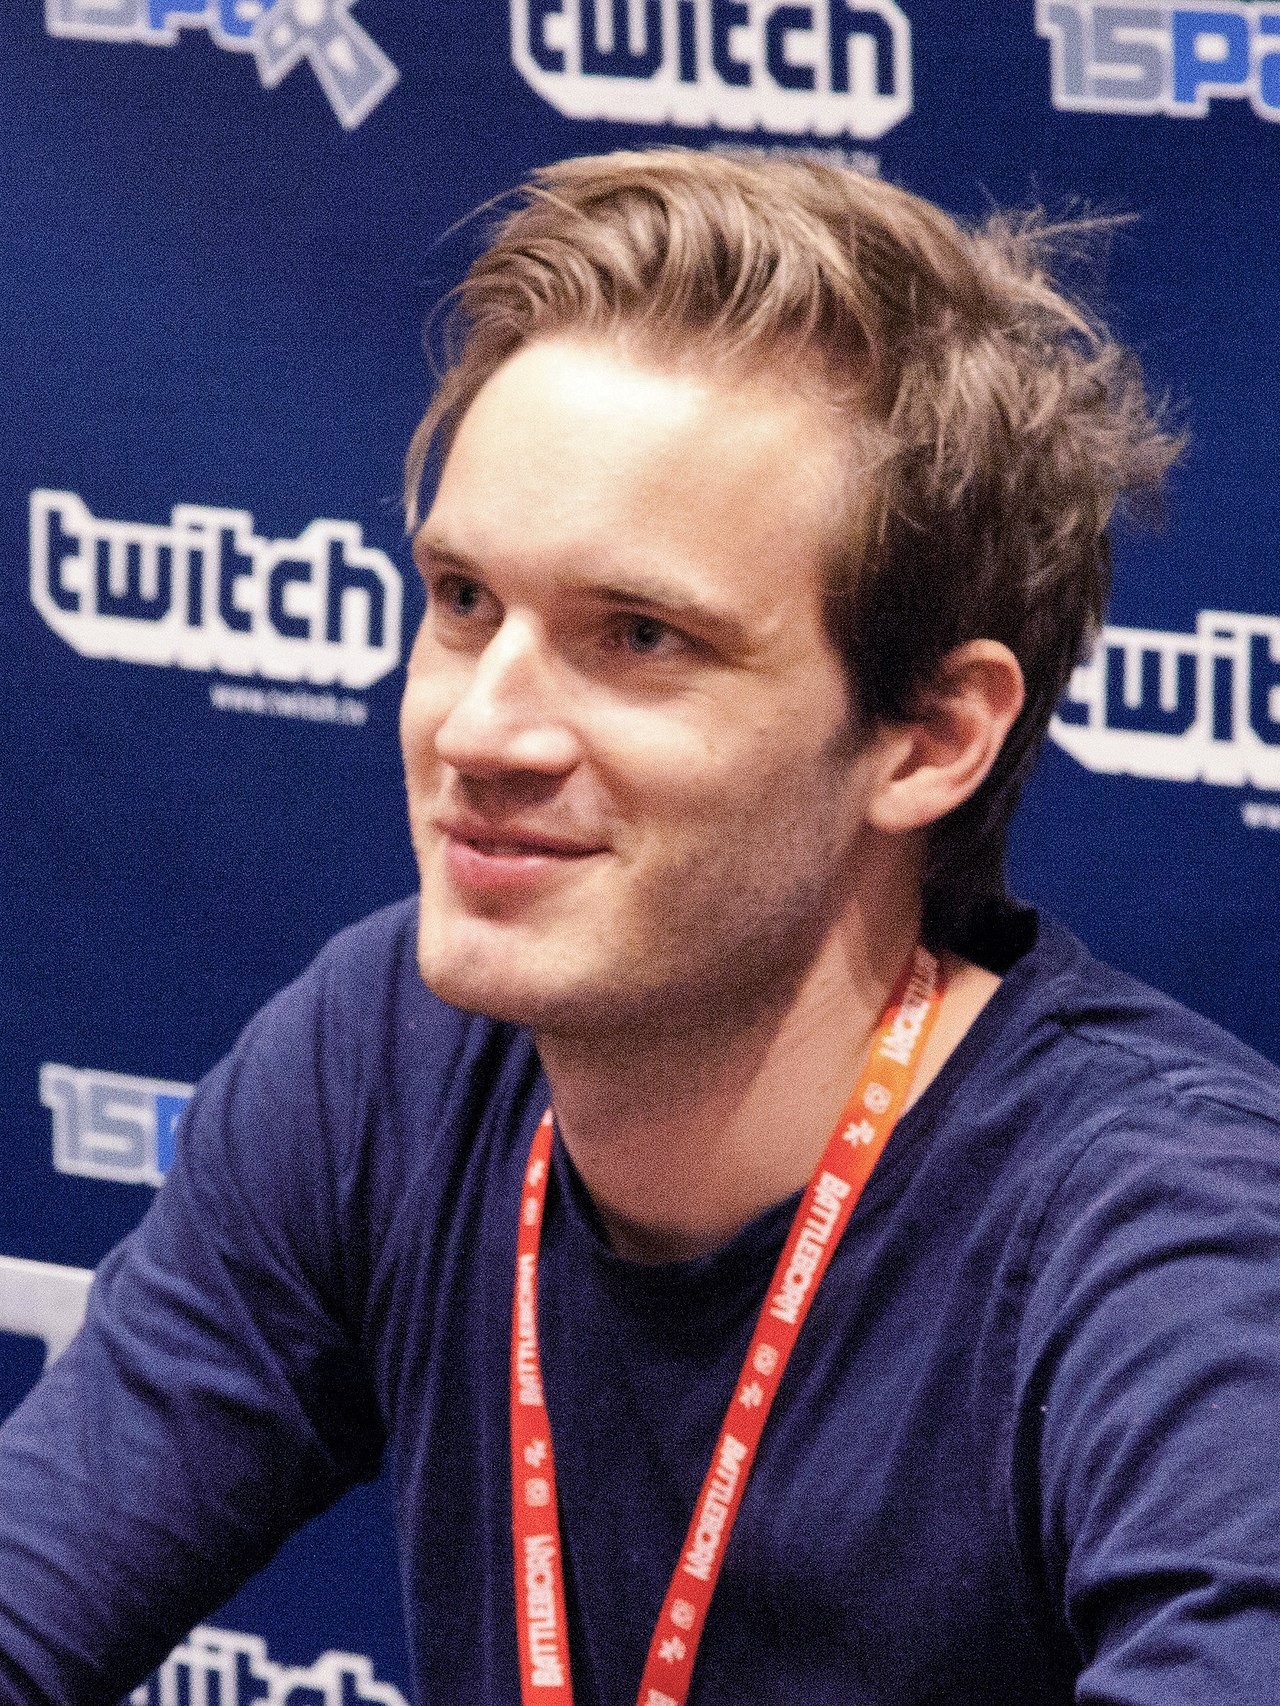
\includegraphics[width=\textwidth]{pewdiepie}
    \caption{Felix "PewDiePie" Kjellberg at PAX 2015.}
  \end{minipage}
\end{figure}

This new policy and YouTube's norm of free performance ran to a head in February of 2017, when \textit{The Wall Street Journal} uncovered a video of famous YouTuber Felix "PewDiePie" Kjellberg reacting to a sign reading "Death to all Jews." This video was the tipping point for many advertisers, causing them to leave YouTube. In response, YouTube stepped up its policy of demonetization across the entirety of its platform, sending ripples through its creator community. For a while, it seemed like the community might hold together despite this. [Alexander 2019]

Then, in 2018, Logan Paul uploaded a horrifying video in which he encountered the body of a man who killed himself in Japan's Aokigahara forest and zoomed in on it in order to draw views to his video. YouTube responded by stepping up its policy of demonetization, dropping many of its small content creators from its Partner Program in a wave known as the "Adpocalypse". YouTubers began to realize that the community was different now, that YouTube was no longer for them. The norms had changed. And so, they begin to leave. In an interview with Logan Paul, famous YouTubers Danny and Michael Philippou said "We leave. We find somewhere else that wants our videos. That used to be YouTube, but it's not anymore. And I don't think it ever will be again." [Alexander 2019]

Massanari, A. 2015. "#Gamergate and The Fappening: How Reddit's Algorithm, Governance, and Culture Support Toxic Technocultures." New Media \& Society, 1-18.\\
 * It is difficult to disentangle community norms from the way they are shaped by the platform itself.

\section{Anonymity and pseudonymity}

Why a section on anonymity? Well, as it turns out, the degree to which you allow your users to remain anonymous is arguably the most important factor which determines your social system's culture.

Before we explore the effects of anonymity, there is a technical point to go over. The "anonymity" you encounter on most social systems (with the exception of a select few services such as the TOR network) isn't technically anonymity but rather pseudonymity. A user is pseudonymous if the user isn't identified by their real name or other common real world identifying features but rather by an alias, such as a username. For a user to be anonymous, there must be no identifying feature of a user -- no alias, nothing. A pseudodnymous user can be traced back to a real world person much more easily than an anonymous user can because all of a pseudonymous user's online activity can be connected to a single pseudonym. By observing the behavior of the pseudonymous user's online activity, one can match the behavior to a real world person's behavior and identify the online user.

Since people commonly refer to pseudonymity as anonymity, to avoid confusion, in this section, when I use the term "anonymity", what I really mean is "pseudonymity" unless I explicitly say otherwise. Now that that technical point is out of the way, let us explore the effects of anonymity on social systems.

One of the biggest effects of anonymity on your social system is how it changes "trolling" and other antisocial behavior on your platform. There is ample evidence showing that allowing users to be anonymous leads to more antisocial behavior such as trolling and cyberbullying [Kiesler et al. 2012]. Users feel less societal pressure to be nice when they can't face any social repercussions for their behavior (their online alias is disliked, not them). They also feel more disconnected from their victims -- their victims are also anonymous and can be dehumanized to some degree.

The downsides to anonymity are certainly great, and great care should be taken whenever considering making part of a social platform anonymous. However, when anonymity is controlled and used thoughtfully, it can be a boon to some social systems. Research has shown that anonymity can lead to stronger communal identity [Ren, Kraut and Kiesler 2012]. Anonymity can also lead individuals to be more creative online than they would in real life [Jessup, Connolly and Galegher 1990].

There are also certain social systems that can only be effectively done if they are anonymous because users need to share personal information. For example, an online LGBTQ+ website might choose to let users be anonymous so that they don't feel like they have to "out" themselves to participate online. An online forum discussing mental health issues might let users be anonymous for similar reasons -- so that they don't feel as scared of sharing their personal stories and asking for help and advice. It is doubly important to make sure these websites are actually anonymous though and that one can't easily connect a user to their real world identity.

Additionally, and perhaps most importantly, in a world in which big tech companies face scandal after scandal for selling user's data to marketing agencies, political organizations and anybody else who can pay, many Internet users have come to place a high value on anonymity. Consider the death of anonymous messaging app Yik Yak for example. While Yik Yak was known by the general public for the cyberbullying that occured on the app (and a few more severe actions, such as bomb threats), many users still signed up for Yik Yak because they wanted an anonymous space. Yik Yak didn't die because of public pressure, at least not directly. Rather, in August of 2016, its creators tried to rehabilitate the app's public image by requiring all users to have usernames, user profiles and verification with real world phone numbers. Suddenly, Yik Yak users became tied to a stable identity, and users began to leave Yik Yak en masse. [Bayne et al. 2019] Consider the following quotes from Yik Yak users, collected by Bayne et al. in 2019:
\begin{center}
"Judging by the fact I can see last weeks post about a million people leave per day."\\
"50,000 people used to live here, now it's a ghost town."\\
"Anonymity was what yik Yak was about. Shame the devs thought otherwise:/"\\
"When they changed it I literally died. I live in hell now."
\end{center}

Helen Nissenbuam sums up many of the benefits of anonymity well in her essay "The Meaning of Anonymity in an Information Age":
\begin{displayquote}
Anonymity may encourage freedom of thought and expression by promising people a possibility to express opinions and develop arguments about positions that, for fear of reprisal or ridicule, they would not or dare not take otherwise. Anonymity may enable people to reach out for help, especially for socially stigmatized problems like domestic violence, HIV or other sexually transmitted infection, emotional problems, or suicidal thoughts. ... It supports socially valuable institutions like peer review, whistle-blowing, and voting.
\end{displayquote}

Again though, it is important to use anonymity \textit{carefully}. It is a powerful tool but with great power comes great responsibility. Many victims of cyberbullying report feeling that social platforms didn't do enough to prevent cyberbullying. They report feeling that even if they reported malicious users, platforms rarely took action against the offenders, leaving the victims to fend for themselves. We want to make successful social platforms. But we don't want to do so at the cost of lives lost, as often happens as a result of cyberbullying. Never prioritize profits over human lives. If you feel your social system can't support scaling up without losing the ability to respond to and prevent cyberbullying, \textit{don't do it}.

\section{Reading questions}

\begin{enumerate}
    \item What is the difference between anonymity and pseudonymity?
    
    \item
    \begin{enumerate}
        \item Bob is a frequent Reddit user who goes by the username \textit{HappyStrongDude9000}. He frequents subreddits such as /r/weightroom and /r/football and often posts his personal take on hot topics and experiences at local establishments (though he doesn't say what city he is from). How might a user find out what city Bob is in?
    \end{enumerate}
\end{enumerate}

\section{Solutions to reading questions}

\begin{enumerate}
    \item You are anonymous if you have no identifier at all. You are pseudonymous if you have a false or placeholder identity.
    
    \item
    \begin{enumerate}
        \item Over time, a user could gather information about Bob such as what his local gym is and what his local sports team is and so on. A user could search for the location of these entities online and find out what city Bob is in.
    \end{enumerate}
\end{enumerate}

\section{Bibliography}

Alexander, Julia. "The Golden Age of YouTube is Over." The Verge. April 5, 2019.

Alkhatib, Ali and Bernstein, Michael. "Street-Level Algorithms: A Theory at the Gaps Between Policy and Decisions." CHI Conference on Human Factors in Computing Systems Proceedings. May 4-9, 2019.

Arthur, Charles and Kiss, Jemima. "Quora: the hottest question-and-answer website you've probably never heard of." \textit{The Guardian}. January 5, 2011.

Bayne, Sian et al. "The social value of anonymity on campus: a study of the decline of Yik Yak." Learning, Media and Technology 44 (2): pp. 92-107. February 27, 2019.

Boyd D. and Hargittai, E. "Facebook Privacy Settings: Who Cares?" First Monday, 15 (8): pp. 13 - 20. 2010.

Burke, Moira et al. "Social use of computer-mediated communication by adults on the autism spectrum." In 2010 ACM Conference on Computer Supported Cooperative Work, CSCW 2010. pp. 425-434. 2010.

Goel, V. "Facebook Tinkers with Users' Emotions in News Feed Experiment, Stirring Outcry." The New York Times. June 29, 2014.

Hull, G. "Successful Failure: What Foucault Can Teach Us about Privacy Self-Management in a World of Facebook and Big Data." Ethics and Information Technology. 2015.

Jessup, Leonard Michael et al. "The effects of anonymity on GDSS group process with an idea-generating task." MIS Quarterly. 14(3):313-321. September, 1990.

Kiesler, Sara et al. "Regulating Behavior in Online Communities." 2012.

Kollock, Peter. "Design Principles for Online Communities." PC Update 15 (5): pp. 58-60. June, 1998.

Lewis, Kevin et al. "The Taste for Privacy: An Analysis of College Student Privacy Settings in an Online Social Network." Journal of Computer-Mediated Communication 14 (1): pp. 79-100. October 1, 2008.

Nissenbaum, Helen. "The Meaning of Anonymity in an Information Age." The Information Society, 15:141-144. 1999.

Ren, Yuqing et al. "Building Member Attachment in Online Communities: Applying Theories of Group Identity and Interpersonal Bonds." MIS Quarterly. 36(3):841-864. September, 2012.

Schleifer, Theodore. "Yes, Quora still exists, and it's now worth \$2 billion." \textit{Vox}. May 16, 2019.

Shontell, Alyson. "Why I Quit My CTO Job At Facebook And Started Quora." \textit{Business Insider}. September 10, 2010.

Spool, Jared. "Do users change their settings?" UIE. September 14, 2011.

Throuvala, Melina A. et al. "Motivational processes and dysfunctional mechanisms of social media use among adolescents: A qualitative focus group study." Computers in Human Behavior. 93:164-175. April, 2019.

Vincent, James. "Twitter taught Microsoft's AI chatbot to be a racist asshole in less than a day." The Verge. March 24, 2016. 

Wilson, James Q. and Kelling, George L. "Broken Windows: The police and neighborhood safety." The Atlantic. March, 1982.

Wondracek, Gilbert et al. "A Practical Attack to De-anonymize Social Network Users." 2010 IEEE Symposium on Security and Privacy. May 16 - 19, 2010.

\end{document}
